\section{微面模型}\label{sec:微面模型}

许多建模表面反射和透射的基于几何光学的方法
都基于一个观点即粗糙表面可以建模为
小的\keyindex{微面}{microfacet}{}合集。
由微面构成的曲面经常建模为高度场\sidenote{译者注:原文heightfield。},
其中微面的朝向分布是作统计上的描述。
\reffig{8.12}展示了相对粗糙表面的横截面和光滑得多的微面表面。
当区别不明显时,我们将用术语\keyindex{微曲面}{microsurface}{}来
描述微面曲面,用\keyindex{宏曲面}{macrosurface}{}来描述基本的光滑曲面
(即由\refvar{Shape}{}表示的)。
\begin{figure}[htbp]
    \centering
    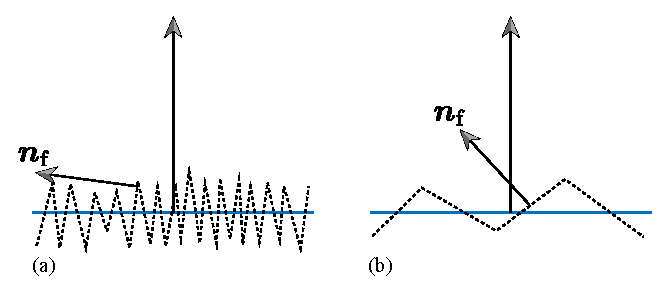
\includegraphics[width=0.75\linewidth]{Pictures/chap08/Roughsmoothmicrofacets.eps}
    \caption{微面曲面模型经常由给出微面法线${\bm n}_{\mathrm{f}}$关于
        曲面法线$\bm n$的分布的函数来描述。(a)微面法线变化越大,表面越粗糙。
        (b)光滑表面的微面法线变化相对较小。}
    \label{fig:8.12}
\end{figure}

基于微面的BRDF模型通过统计上对来自大量微面的光的散射建模来奏效。
如果我们假设被照明的微分区域$\mathrm{d}A$比起单个微面的尺寸相对大些,
则有大量微面被照亮且它们合起来的表现决定了观察到的散射。

微面模型的两个主要构成是\keyindex{刻面}{facet}{}
\sidenote{译者注:暂未查到facet在图形学中的专门翻译。}分布的表示
和描述光如何从单个微面散射的BRDF。有了这些,
任务是推导BRDF的解析表达式以描述来自这类曲面的散射。
尽管镜面透射对于建模许多透明材料很有用,
但对于微面BRDF,完美镜面反射是最常用的,
(下节介绍的)Oren-Nayar模型把微面看作朗伯反射体。

为了计算来自这类模型的反射,需要考虑微面级的局部光效应(\reffig{8.13})。
微面可能被另一刻面遮挡,可能处在相邻微面的阴影下,
或者\keyindex{互反射}{interreflection}{}可能
造成微面反射出比直接照明量和低层级微面BRDF预计的还多的光。
基于微面的特定BRDF模型以各种精确程度考虑了这些效应的每一种。
一般方法是做出尽可能最好的近似,且仍得到计算简单的表达式。
\begin{figure}[htbp]
    \centering
    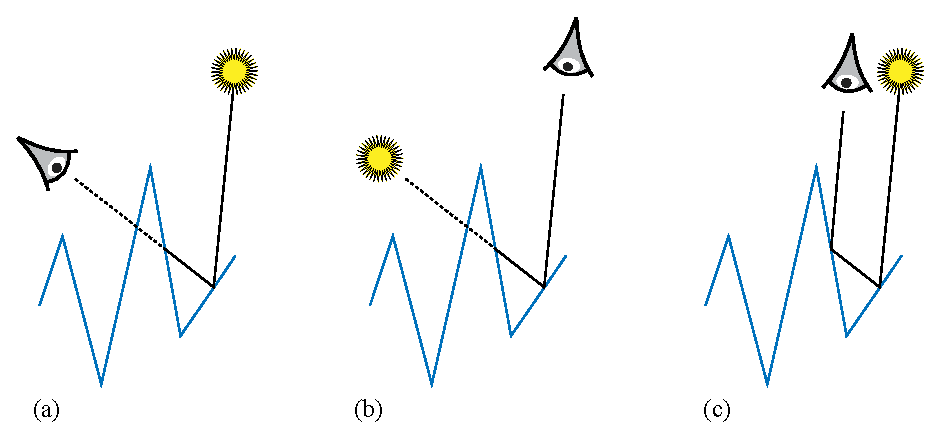
\includegraphics[width=\linewidth]{Pictures/chap08/Maskingshadowinginterreflection.eps}
    \caption{微面反射模型要考虑的三种重要几何效应。(a)遮掩(masking):
        考虑的微面因为另一微面的遮挡而对观察者不可见。(b)阴影(shadowing):
        类似地,光无法到达微面。(3)互反射:光在到达
        观察者之前于微面之间反弹。}
    \label{fig:8.13}
\end{figure}

\subsection{Oren-Nayar漫反射}\label{sub:Oren-Nayar漫反射}
\citet{10.1145/192161.192213}观察到真实世界物体不会展现完美朗伯反射。
具体地,当照明方向接近观察方向时,粗糙曲面通常显得更亮。
他们用含有单个参数$\sigma$即微面朝向角度标准差的球面高斯分布
描述的V形微面构建了描述粗糙曲面的反射模型。

在V形假设下,可以通过只考虑相邻微面来处理互反射;
\citeauthor{10.1145/192161.192213}利用这点
推导出对凹槽\sidenote{译者注:原文groove。}集的整体反射建模的BRDF。

所得模型考虑了微面间的阴影、遮掩和互反射,但没有解析解,
所以他们发现下列近似拟合得很好:
\begin{align*}
    f_{\mathrm{r}}({\bm\omega}_{\mathrm{i}},{\bm\omega}_{\mathrm{o}})=\frac{R}{\pi}(A+B\max(0,\cos(\varphi_{\mathrm{i}}-\varphi_{\mathrm{o}}))\sin\alpha\tan\beta)\, ,
\end{align*}
其中如果$\sigma$单位是弧度,则
\begin{align*}
    A      & =1-\frac{\sigma^2}{2(\sigma^2+0.33)}\, ,           \\
    B      & =\frac{0.45\sigma^2}{\sigma^2+0.09}\, ,            \\
    \alpha & =\max(\theta_{\mathrm{i}},\theta_{\mathrm{o}})\, , \\
    \beta  & =\min(\theta_{\mathrm{i}},\theta_{\mathrm{o}})\, .
\end{align*}

\begin{figure}[htbp]
    \centering
    \subfloat[朗伯]{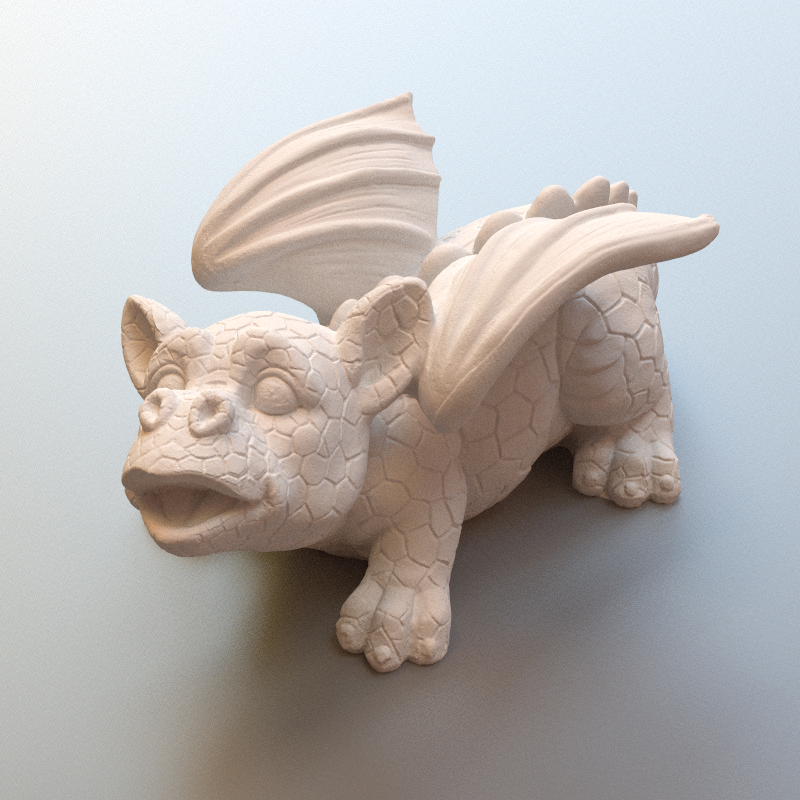
\includegraphics[width=0.7\linewidth]{Pictures/chap08/f8-14a.png}\label{fig:8.14.1}}\\
    \subfloat[Oren-Nayar]{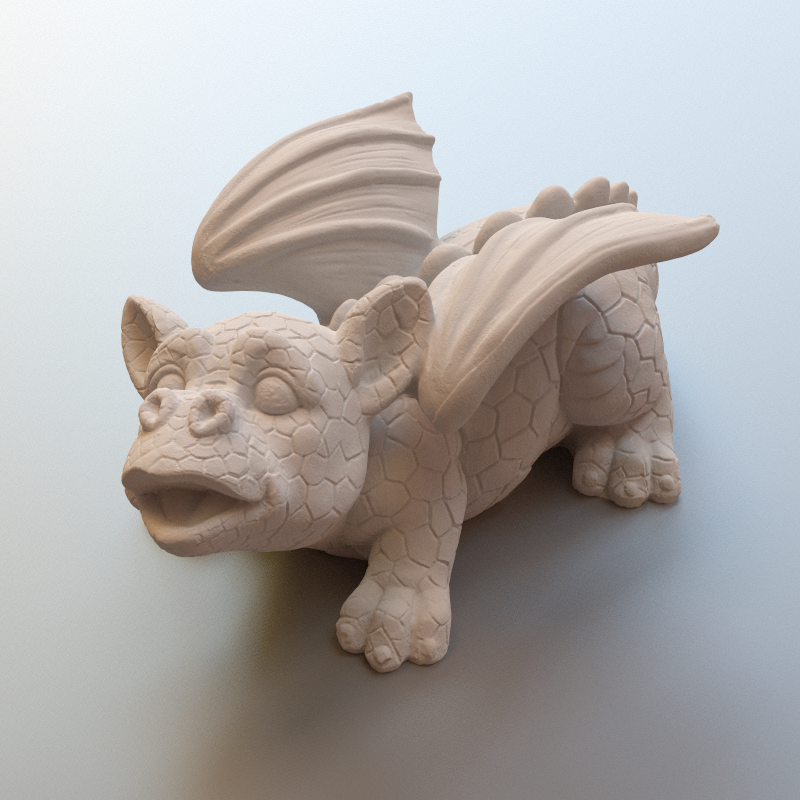
\includegraphics[width=0.7\linewidth]{Pictures/chap08/f8-14b.png}\label{fig:8.14.2}}
    \caption{(a)来自\refvar{LambertianReflection}{}模型的标准漫反射和
        (b)$\sigma$参数为20度的\refvar{OrenNayar}{}模型渲染的龙模型。
        注意用Oren-Nayar模型时暗色轮廓边缘反射增加了,浅色明暗边缘通常也更干脆
        (感谢Christian Schüller提供的模型)。}
    \label{fig:8.14}
\end{figure}

这里的实现在构造函数中预先计算和保存参数$A$与$B$的值
以节约稍后计算BRDF的工作量。\reffig{8.14}比较了理想漫反射和Oren-Nayar模型渲染的区别。
\begin{lstlisting}
`\initcode{OrenNayar Public Methods}{=}`
`\initvar{OrenNayar}{}`(const `\refvar{Spectrum}{}` &R, `\refvar{Float}{}` sigma) 
    : `\refvar{BxDF}{}`(`\refvar{BxDFType}{}`(`\refvar[BSDFREFLECTION]{BSDF\_REFLECTION}{}` | `\refvar[BSDFDIFFUSE]{BSDF\_DIFFUSE}{}`)), `\refvar[OrenNayar::R]{R}{}`(R) {
    sigma = `\refvar{Radians}{}`(sigma);
    `\refvar{Float}{}` sigma2 = sigma * sigma;
    `\refvar[OrenNayar::A]{A}{}` = 1.f - (sigma2 / (2.f * (sigma2 + 0.33f)));
    `\refvar[OrenNayar::B]{B}{}` = 0.45f * sigma2 / (sigma2 + 0.09f);
}
\end{lstlisting}
\begin{lstlisting}
`\initcode{OrenNayar Private Data}{=}`
const `\refvar{Spectrum}{}` `\initvar[OrenNayar::R]{R}{}`;
`\refvar{Float}{}` `\initvar[OrenNayar::A]{A}{}`, `\initvar[OrenNayar::B]{B}{}`;
\end{lstlisting}

比起直接变换基本方程,三角恒等式的应用可以极大提升求值例程的效率。
实现从计算$\sin\theta_{\mathrm{i}}$和$\sin\theta_{\mathrm{o}}$的值开始。
\begin{lstlisting}
`\refcode{BxDF Method Definitions}{+=}\lastnext{BxDFMethodDefinitions}`
`\refvar{Spectrum}{}` `\refvar{OrenNayar}{}`::`\initvar[OrenNayar::f]{f}{}`(const `\refvar{Vector3f}{}` &wo, const `\refvar{Vector3f}{}` &wi) const {
    `\refvar{Float}{}` sinThetaI = `\refvar{SinTheta}{}`(wi);
    `\refvar{Float}{}` sinThetaO = `\refvar{SinTheta}{}`(wo);
    `\refcode{Compute cosine term of Oren-Nayar model}{}`
    `\refcode{Compute sine and tangent terms of Oren-Nayar model}{}`
    return `\refvar[OrenNayar::R]{R}{}` * `\refvar{InvPi}{}` * (`\refvar[OrenNayar::A]{A}{}` + `\refvar[OrenNayar::B]{B}{}` * maxCos * sinAlpha * tanBeta);
}
\end{lstlisting}

为了计算项$\max(0,\cos(\varphi_{\mathrm{i}}-\varphi_{\mathrm{o}}))$,
我们可以应用三角恒等式
\begin{align*}
    \cos(a-b)=\cos a\cos b+\sin a\sin b\, ,
\end{align*}
这样我们只需要计算$\varphi_{\mathrm{i}}$和$\varphi_{\mathrm{o}}$的正弦和余弦。
\begin{lstlisting}
`\initcode{Compute cosine term of Oren-Nayar model}{=}`
`\refvar{Float}{}` maxCos = 0;
if (sinThetaI > 1e-4 && sinThetaO > 1e-4) {
    `\refvar{Float}{}` sinPhiI = `\refvar{SinPhi}{}`(wi), cosPhiI = `\refvar{CosPhi}{}`(wi);
    `\refvar{Float}{}` sinPhiO = `\refvar{SinPhi}{}`(wo), cosPhiO = `\refvar{CosPhi}{}`(wo);
    `\refvar{Float}{}` dCos = cosPhiI * cosPhiO + sinPhiI * sinPhiO;
    maxCos = std::max((`\refvar{Float}{}`)0, dCos);
}
\end{lstlisting}

最后,求得项$\sin\alpha$和$\tan\beta$.
注意无论${\bm\omega}_{\mathrm{i}}$或${\bm\omega}_{\mathrm{o}}$中的哪一个,
有更大的$\cos\theta$(即更大的$z$分量)就有更小的$\theta$.
我们可以用该方法开头计算的近似正弦值来设定$\sin\alpha$.
然后用恒等式$\displaystyle\tan\theta=\frac{\sin\theta}{\cos\theta}$计算正切。
\begin{lstlisting}
`\initcode{Compute sine and tangent terms of Oren-Nayar model}{=}`
`\refvar{Float}{}` sinAlpha, tanBeta;
if (`\refvar{AbsCosTheta}{}`(wi) > `\refvar{AbsCosTheta}{}`(wo)) {
    sinAlpha = sinThetaO;
    tanBeta = sinThetaI / `\refvar{AbsCosTheta}{}`(wi);
} else {
    sinAlpha = sinThetaI;
    tanBeta = sinThetaO / `\refvar{AbsCosTheta}{}`(wo);
}
\end{lstlisting}

\subsection{微面分布函数}\label{sub:微面分布函数}
反射模型所基于的微面展现完美镜面反射和透射时,
其对来自各种光泽材料的光散射的建模已经很高效了,包括金属、塑料和磨砂玻璃。
